% Native TikZ figures for Banks QFT Appendix D.
% BANKS-SOURCE: pdf=261 print=251 kind=figure id=appendixD-propagator-gauge
% BANKS-SOURCE: pdf=262 print=252 kind=figure id=appendixD-propagator-ghost-fermi
% BANKS-SOURCE: pdf=262 print=252 kind=figure id=appendixD-vertex-fermion-gauge
% BANKS-SOURCE: pdf=262 print=252 kind=figure id=appendixD-vertex-three-gauge
% BANKS-SOURCE: pdf=263 print=253 kind=figure id=appendixD-vertices-four-through-scalar
% BANKS-SOURCE: pdf=265 print=255 kind=figure id=figure-D.1

\tikzset{
  BanksDLine/.style={line width=0.62pt, line cap=round, line join=round},
  % Gauge-boson lines.  The stand-alone propagator in the source is a lazy
  % sine; the wavy legs of the vertices are a tight spring.
  BanksDPhotonLong/.style={BanksDLine, decorate,
    decoration={snake, amplitude=2.1pt, segment length=13.0pt}},
  BanksDPhoton/.style={BanksDLine, decorate,
    decoration={snake, amplitude=2.3pt, segment length=5.0pt}},
  BanksDGluon/.style={BanksDLine, decorate,
    decoration={coil, amplitude=6.0pt, segment length=20.0pt, aspect=0.85}},
  % Scalars: dashed.  Ghosts: dashed with a finer pattern (source p.252/253).
  BanksDScalar/.style={BanksDLine, dash pattern=on 5.0pt off 4.2pt},
  BanksDGhost/.style={BanksDLine, dash pattern=on 3.5pt off 2.8pt},
  BanksDFermion/.style={BanksDLine},
  BanksDArrow/.style={postaction={decorate,
    decoration={markings, mark=at position 0.52 with {\arrow{Stealth[length=5.0pt,width=4.0pt]}}}}},
  BanksDEveryNode/.style={font=\small},
}

% Propagators -----------------------------------------------------------------

\newcommand{\BanksDGaugePropagator}{%
  \par\nobreak{\centering
  \resizebox{0.82\textwidth}{!}{%
  \begin{tikzpicture}[x=1cm,y=1cm,BanksDEveryNode]
    \draw[BanksDPhotonLong] (-4.3,0) -- (-1.6,0);
    \node[anchor=west] at (-0.9,0) {$\displaystyle
      \frac{-\mathrm{i}\!\left(\eta_{\mu\nu}
      -\dfrac{p_\mu p_\nu(1-\kappa)}
      {p^2+\kappa m_A^2-\mathrm{i}\epsilon}\right)}
      {p^2+m_A^2-\mathrm{i}\epsilon}$};
    \node[anchor=west] at (3.85,0) {$\displaystyle
      \frac{\delta_{AB}
      -\dfrac{p_{EA}p_{EB}(1-\kappa)}
      {p_E^2+\kappa m_A^2}}
      {p_E^2+m_A^2}$};
  \end{tikzpicture}%
  }\par}%
}

\newcommand{\BanksDGluonLine}{%
  \begin{center}
  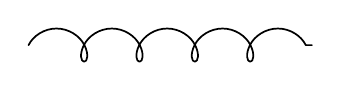
\begin{tikzpicture}[x=1cm,y=1cm]
    \draw[BanksDGluon] (-1.8,0) -- (1.8,0);
  \end{tikzpicture}
  \end{center}%
}

\newcommand{\BanksDScalarPropagator}{%
  \par\nobreak{\centering
  \resizebox{0.82\textwidth}{!}{%
  \begin{tikzpicture}[x=1cm,y=1cm,BanksDEveryNode]
    \draw[BanksDScalar,BanksDArrow] (-4.3,0) -- (-1.6,0);
    \node[anchor=west] at (-0.9,0) {$\displaystyle
      \frac{-\mathrm{i}}{p^2+m_S^2-\mathrm{i}\epsilon}$};
    \node[anchor=west] at (3.25,0) {$\displaystyle
      \frac{1}{p_E^2+m_S^2}$};
  \end{tikzpicture}%
  }\par}%
}

\newcommand{\BanksDGhostPropagator}{%
  \par\nobreak{\centering
  \resizebox{0.82\textwidth}{!}{%
  \begin{tikzpicture}[x=1cm,y=1cm,BanksDEveryNode]
    \draw[BanksDGhost,BanksDArrow] (-4.3,0) -- (-1.6,0);
    \node[anchor=west] at (-0.9,0) {$\displaystyle
      \frac{-\mathrm{i}}{p^2+\kappa m_V^2-\mathrm{i}\epsilon}$};
    \node[anchor=west] at (3.25,0) {$\displaystyle
      \frac{1}{p_E^2+\kappa m_V^2}$};
  \end{tikzpicture}%
  }\par}%
}

\newcommand{\BanksDFermionPropagator}{%
  \par\nobreak{\centering
  \resizebox{0.82\textwidth}{!}{%
  \begin{tikzpicture}[x=1cm,y=1cm,BanksDEveryNode]
    \draw[BanksDFermion,BanksDArrow] (-4.3,0) -- (-1.6,0);
    \node[anchor=west] at (-0.9,0) {$\displaystyle
      \frac{-\mathrm{i}(\slashed p+m_F)}
      {p^2+m_F^2-\mathrm{i}\epsilon}$};
    \node[anchor=west] at (3.25,0) {$\displaystyle
      \frac{1}{\slashed p_E+\mathrm{i}m_F}$};
  \end{tikzpicture}%
  }\par}%
}

% Vertices --------------------------------------------------------------------

% Fermion flow runs through the vertex: in from the upper left, out to the
% upper right (source p.252).
\newcommand{\BanksDFermionGaugeVertex}{%
  \begin{center}
  \begin{tikzpicture}[x=1cm,y=1cm,BanksDEveryNode]
    \draw[BanksDFermion,BanksDArrow] (-1.20,1.40) -- (0,0);
    \draw[BanksDFermion,BanksDArrow] (0,0) -- (1.20,1.40);
    \draw[BanksDPhoton] (0,0) -- (0,-1.30);
    \node[anchor=west] at (3.1,0.15) {$\mathrm{i}g\gamma^\mu T_F^aP$
      \hspace{1.0em} $-g\gamma_E^A T_F^aP$};
  \end{tikzpicture}
  \end{center}%
}

\newcommand{\BanksDThreeGaugeVertex}{%
  \begin{center}
  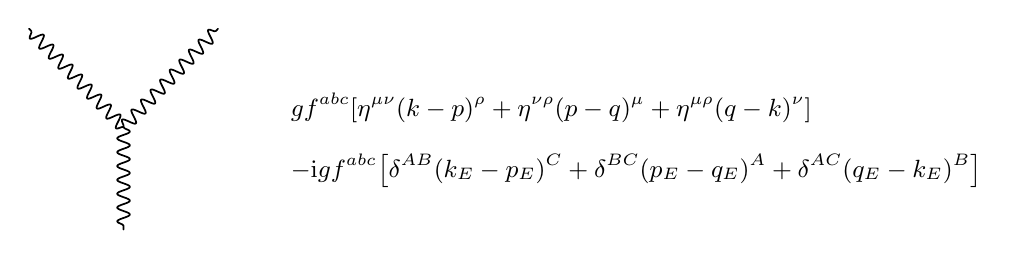
\begin{tikzpicture}[x=1cm,y=1cm,BanksDEveryNode]
    \draw[BanksDPhoton] (0,0) -- (-1.20,1.25);
    \draw[BanksDPhoton] (0,0) -- (1.20,1.25);
    \draw[BanksDPhoton] (0,0) -- (0,-1.30);
    \node[anchor=west] at (2.0,0.25) {$\displaystyle
      g f^{abc}\!\left[\eta^{\mu\nu}(k-p)^\rho
      +\eta^{\nu\rho}(p-q)^\mu
      +\eta^{\mu\rho}(q-k)^\nu\right]$};
    \node[anchor=west] at (2.0,-0.55) {$\displaystyle
      -\mathrm{i}g f^{abc}\!\left[\delta^{AB}(k_E-p_E)^C
      +\delta^{BC}(p_E-q_E)^A
      +\delta^{AC}(q_E-k_E)^B\right]$};
  \end{tikzpicture}
  \end{center}%
}

\newcommand{\BanksDFourGaugeVertex}{%
  \begin{center}
  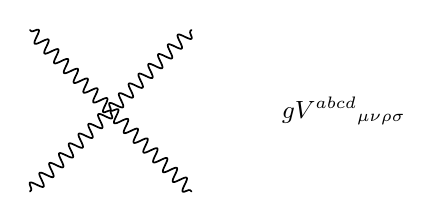
\begin{tikzpicture}[x=1cm,y=1cm,BanksDEveryNode]
    \foreach \ang in {45,135,225,315} {
      \draw[BanksDPhoton] (0,0) -- (\ang:1.45);
    }
    \node[anchor=west] at (2.05,0) {$gV^{abcd}{}_{\mu\nu\rho\sigma}$};
  \end{tikzpicture}
  \end{center}%
}

\newcommand{\BanksDFourGaugeFormula}{%
  \begin{equation*}
    \begin{aligned}
      V^{abcd}{}_{\mu\nu\rho\sigma}
      ={}&-\mathrm{i}g^2\bigl[ f^{abe}f^{cde}
      (\eta^{\mu\rho}\eta^{\nu\sigma}
      -\eta^{\nu\rho}\eta^{\mu\sigma})\\[-2pt]
      &\quad+ f^{ace}f^{bde}
      (\eta^{\mu\nu}\eta^{\rho\sigma}
      -\eta^{\nu\rho}\eta^{\mu\sigma})\\[-2pt]
      &\quad+ f^{ade}f^{bce}
      (\eta^{\mu\nu}\eta^{\rho\sigma}
      -\eta^{\mu\rho}\eta^{\nu\sigma})\bigr].
    \end{aligned}
  \end{equation*}%
}

% Both ghost arrows point into the vertex in the source (p.253).
\newcommand{\BanksDGhostGaugeVertex}{%
  \begin{center}
  \begin{tikzpicture}[x=1cm,y=1cm,BanksDEveryNode]
    \draw[BanksDGhost,BanksDArrow] (-1.20,1.35) -- (0,0);
    \draw[BanksDGhost,BanksDArrow] (1.20,1.35) -- (0,0);
    \draw[BanksDPhoton] (0,0) -- (0,-1.30);
    \node[anchor=west] at (2.0,0.08) {$g f^{abc}p^\mu$
      \hspace{1.0em} $-\mathrm{i}g f^{abc}p_E^A$};
  \end{tikzpicture}
  \end{center}%
}

\newcommand{\BanksDYukawaVertex}{%
  \begin{center}
  \begin{tikzpicture}[x=1cm,y=1cm,BanksDEveryNode]
    \draw[BanksDFermion,BanksDArrow] (-1.20,1.35) -- (0,0);
    \draw[BanksDFermion,BanksDArrow] (0,0) -- (1.20,1.35);
    \draw[BanksDScalar] (0,0) -- (0,-1.30);
    \node[anchor=west] at (2.0,0.08) {$-\mathrm{i}gM$
      \hspace{1.65em} $gM$};
  \end{tikzpicture}
  \end{center}%
}

\newcommand{\BanksDScalarGaugeVertex}{%
  \begin{center}
  \begin{tikzpicture}[x=1cm,y=1cm,BanksDEveryNode]
    \draw[BanksDFermion,BanksDArrow] (-1.25,1.35) -- (0,0);
    \draw[BanksDFermion,BanksDArrow] (0,0) -- (1.25,1.35);
    \draw[BanksDPhoton] (0,0) -- (0,-1.35);
    \node[anchor=west] at (2.0,0.06) {$\displaystyle
      -\mathrm{i}g(p+p')^\mu T_S^aP$
      \hspace{0.85em} $\displaystyle g(p_E+p_E')^A T_S^a$};
  \end{tikzpicture}
  \end{center}%
}

\newcommand{\BanksDScalarScalarGaugeVertex}{%
  \begin{center}
  \begin{tikzpicture}[x=1cm,y=1cm,BanksDEveryNode]
    \draw[BanksDFermion,BanksDArrow] (-1.25,1.40) -- (0,0);
    \draw[BanksDFermion,BanksDArrow] (0,0) -- (1.25,1.40);
    \draw[BanksDPhoton] (0,0) -- (-1.15,-1.35);
    \draw[BanksDPhoton] (0,0) -- (1.15,-1.35);
    \node[anchor=west] at (2.0,0.08) {$\displaystyle
      \mathrm{i}g[T_S^a,T_S^b]_+\eta^{\mu\nu}$
      \hspace{0.85em} $\displaystyle -g[T_S^a,T_S^b]_+\delta^{AB}$};
  \end{tikzpicture}
  \end{center}%
}

% Figure D.1 ------------------------------------------------------------------
%
% Each row of the source figure shows the ten fields of the Wick expansion,
% the contractions drawn as brackets above and below the line, the resulting
% graph, and the combinatoric factor.  The field tokens are laid out as named
% nodes so that every bracket lands on the field it actually contracts.

\tikzset{
  BanksDFld/.style={anchor=base west, inner sep=0pt, outer sep=0pt},
}

% Vertical reference levels for the bracket stems and bars.
\def\BanksDFldBase{1.35}
\def\BanksDTopFoot{1.55}
\def\BanksDBotFoot{1.22}
\def\BanksDStep{0.11}

\newcommand{\BanksDFields}{%
  \node[BanksDFld] (fx)  at (0,\BanksDFldBase) {$\phi(\mathrm{x})$};
  \node[BanksDFld] (fy)  at (fx.base east)  {$\phi(\mathrm{y})$};
  \node[BanksDFld] (fiw) at (fy.base east)  {$\;\int\! \dd^D w\;$};
  \node[BanksDFld] (fw1) at (fiw.base east) {$\phi(\mathrm{w})$};
  \node[BanksDFld] (fw2) at (fw1.base east) {$\phi(\mathrm{w})$};
  \node[BanksDFld] (fw3) at (fw2.base east) {$\phi(\mathrm{w})$};
  \node[BanksDFld] (fw4) at (fw3.base east) {$\phi(\mathrm{w})$};
  \node[BanksDFld] (fiz) at (fw4.base east) {$\;\int\! \dd^D z\;$};
  \node[BanksDFld] (fz1) at (fiz.base east) {$\phi(\mathrm{z})$};
  \node[BanksDFld] (fz2) at (fz1.base east) {$\phi(\mathrm{z})$};
  \node[BanksDFld] (fz3) at (fz2.base east) {$\phi(\mathrm{z})$};
  \node[BanksDFld] (fz4) at (fz3.base east) {$\phi(\mathrm{z})$};
}

% #1 = left field node, #2 = right field node, #3 = nesting level (0 = innermost)
\newcommand{\BanksDTopB}[3]{%
  \pgfmathsetmacro{\BanksDBar}{\BanksDTopFoot+\BanksDStep*(#3+1)}%
  \draw[BanksDLine]
    (#1.west |- 0,\BanksDTopFoot) -- (#1.west |- 0,\BanksDBar)
    -- (#2.east |- 0,\BanksDBar) -- (#2.east |- 0,\BanksDTopFoot);
}
\newcommand{\BanksDBotB}[3]{%
  \pgfmathsetmacro{\BanksDBar}{\BanksDBotFoot-\BanksDStep*(#3+1)}%
  \draw[BanksDLine]
    (#1.west |- 0,\BanksDBotFoot) -- (#1.west |- 0,\BanksDBar)
    -- (#2.east |- 0,\BanksDBar) -- (#2.east |- 0,\BanksDBotFoot);
}

% Graph primitives.  A vertex dot with its label underneath.
\newcommand{\BanksDDot}[3]{%
  \fill (#1,#2) circle (1.6pt);
  \node[anchor=north,inner sep=1.5pt] at (#1,{#2-0.20}) {$#3$};
}
\newcommand{\BanksDPlainDot}[2]{\fill (#1,#2) circle (1.6pt);}

% A tadpole sitting on top of the vertex.
\newcommand{\BanksDSelfLoop}[2]{%
  \draw[BanksDLine] (#1,{#2+0.22}) ellipse[x radius=0.13,y radius=0.22];
}
% Two tadpoles, one above and one below (the figure-eight of the source).
\newcommand{\BanksDDoubleSelfLoop}[2]{%
  \draw[BanksDLine] (#1,{#2+0.22}) ellipse[x radius=0.13,y radius=0.22];
  \draw[BanksDLine] (#1,{#2-0.22}) ellipse[x radius=0.13,y radius=0.22];
}

\newcommand{\BanksDTwoParallel}[3]{%
  \draw[BanksDLine] (#1,#3) .. controls ({#1+0.30},{#3+0.30})
    and ({#2-0.30},{#3+0.30}) .. (#2,#3);
  \draw[BanksDLine] (#1,#3) .. controls ({#1+0.30},{#3-0.30})
    and ({#2-0.30},{#3-0.30}) .. (#2,#3);
}
\newcommand{\BanksDThreeParallel}[3]{%
  \draw[BanksDLine] (#1,#3) -- (#2,#3);
  \BanksDTwoParallel{#1}{#2}{#3}%
}
\newcommand{\BanksDFourParallel}[3]{%
  \foreach \BanksDOff in {-0.34,-0.11,0.11,0.34} {
    \draw[BanksDLine] (#1,#3) .. controls ({#1+0.26},{#3+\BanksDOff})
      and ({#2-0.26},{#3+\BanksDOff}) .. (#2,#3);
  }
}

\newcommand{\BanksDFactor}[1]{%
  \node[anchor=west] at (7.0,0) {$\displaystyle #1$};
}

\newcommand{\BanksDCombinatoricFigure}{%
  \resizebox{0.82\textwidth}{!}{%
  \begin{tikzpicture}[
    x=1cm,y=1cm,
    every node/.style={font=\small},
    line cap=round,line join=round]

    % Row 1: x-y propagator; two self-contracted quartic vertices.
    % Contractions: (x y)(w1 w2)(w3 w4)(z1 z2)(z3 z4).
    \begin{scope}[yshift=0cm]
      \BanksDFields
      \BanksDTopB{fx}{fy}{0}
      \BanksDTopB{fw1}{fw2}{0}
      \BanksDTopB{fw3}{fw4}{0}
      \BanksDTopB{fz1}{fz2}{0}
      \BanksDTopB{fz3}{fz4}{0}
      \draw[BanksDLine] (0.8,0) -- (1.9,0);
      \BanksDDot{0.8}{0}{x}\BanksDDot{1.9}{0}{y}
      \BanksDDoubleSelfLoop{3.1}{0}\BanksDDoubleSelfLoop{4.3}{0}
      \BanksDDot{3.1}{0}{w}\BanksDDot{4.3}{0}{z}
      \BanksDFactor{\frac{3^2}{2\cdot(4!)^2}=\frac{1}{128}}
    \end{scope}

    % Row 2: one self-contraction at each vertex, two lines between them.
    % Contractions: (x y)(w1 w2)(w3 z1)(w4 z2)(z3 z4).
    \begin{scope}[yshift=-2.55cm]
      \BanksDFields
      \BanksDTopB{fx}{fy}{0}
      \BanksDTopB{fw1}{fw2}{0}
      \BanksDTopB{fw3}{fz1}{1}
      \BanksDTopB{fz3}{fz4}{0}
      \BanksDBotB{fw4}{fz2}{0}
      \draw[BanksDLine] (0.8,0) -- (1.9,0);
      \BanksDDot{0.8}{0}{x}\BanksDDot{1.9}{0}{y}
      \BanksDTwoParallel{3.1}{4.4}{0}
      \BanksDSelfLoop{3.1}{0}\BanksDSelfLoop{4.4}{0}
      \BanksDDot{3.1}{0}{w}\BanksDDot{4.4}{0}{z}
      \BanksDFactor{\frac{2\cdot\binom{4}{2}^{\!2}}{2\cdot(4!)^2}=\frac{1}{16}}
    \end{scope}

    % Row 3: four lines joining the two vertices.
    % Contractions: (x y)(w1 z4)(w2 z3)(w3 z2)(w4 z1).
    \begin{scope}[yshift=-5.10cm]
      \BanksDFields
      \BanksDTopB{fx}{fy}{0}
      \BanksDTopB{fw1}{fz4}{1}
      \BanksDTopB{fw2}{fz3}{0}
      \BanksDBotB{fw3}{fz2}{1}
      \BanksDBotB{fw4}{fz1}{0}
      \draw[BanksDLine] (0.8,0) -- (1.9,0);
      \BanksDDot{0.8}{0}{x}\BanksDDot{1.9}{0}{y}
      \BanksDFourParallel{3.1}{4.6}{0}
      \BanksDDot{3.1}{0}{w}\BanksDDot{4.6}{0}{z}
      \BanksDFactor{\frac{4!}{2\cdot(4!)^2}=\frac{1}{48}}
    \end{scope}

    % Row 4: x-w-y chain with a tadpole at w; z self-contracts twice.
    % Contractions: (x w1)(y w2)(w3 w4)(z1 z2)(z3 z4).
    \begin{scope}[yshift=-7.65cm]
      \BanksDFields
      \BanksDTopB{fx}{fw1}{0}
      \BanksDTopB{fw3}{fw4}{0}
      \BanksDTopB{fz1}{fz2}{0}
      \BanksDTopB{fz3}{fz4}{0}
      \BanksDBotB{fy}{fw2}{0}
      \draw[BanksDLine] (0.8,0) -- (3.4,0);
      \BanksDSelfLoop{2.1}{0}
      \BanksDDot{0.8}{0}{x}\BanksDDot{2.1}{0}{w}\BanksDDot{3.4}{0}{y}
      \BanksDDoubleSelfLoop{4.6}{0}
      \BanksDDot{4.6}{0}{z}
      \BanksDFactor{\frac{2\cdot4\cdot3\cdot3}{2\cdot(4!)^2}=\frac{1}{16}}
    \end{scope}

    % Row 5: x and y both attach to w; two lines w-z; tadpole at z.
    % Contractions: (x w1)(y w2)(w3 z1)(w4 z2)(z3 z4).
    \begin{scope}[yshift=-10.20cm]
      \BanksDFields
      \BanksDTopB{fx}{fw1}{0}
      \BanksDTopB{fw3}{fz1}{0}
      \BanksDTopB{fz3}{fz4}{0}
      \BanksDBotB{fy}{fw2}{0}
      \BanksDBotB{fw4}{fz2}{0}
      \draw[BanksDLine] (0.8,0.30) -- (2.4,0);
      \draw[BanksDLine] (0.8,-0.30) -- (2.4,0);
      \BanksDTwoParallel{2.4}{4.0}{0}
      \BanksDSelfLoop{4.0}{0}
      \BanksDPlainDot{0.8}{0.30}\BanksDPlainDot{0.8}{-0.30}
      \node[anchor=east,inner sep=2.5pt] at (0.8,0.30) {$x$};
      \node[anchor=east,inner sep=2.5pt] at (0.8,-0.30) {$y$};
      \BanksDDot{2.4}{0}{w}\BanksDDot{4.0}{0}{z}
      \BanksDFactor{\frac{2\cdot4\cdot3\cdot2\cdot\binom{4}{2}}{2\cdot(4!)^2}=\frac{1}{4}}
    \end{scope}

    % Row 6: y-w-z-x chain with a tadpole at w and one at z.
    % Contractions: (y w1)(w2 w3)(w4 z1)(z2 z3)(x z4).
    \begin{scope}[yshift=-12.75cm]
      \BanksDFields
      \BanksDTopB{fy}{fw1}{0}
      \BanksDTopB{fw2}{fw3}{0}
      \BanksDTopB{fw4}{fz1}{0}
      \BanksDTopB{fz2}{fz3}{0}
      \BanksDBotB{fx}{fz4}{0}
      \draw[BanksDLine] (0.8,0) -- (4.4,0);
      \BanksDSelfLoop{2.0}{0}\BanksDSelfLoop{3.2}{0}
      \BanksDDot{0.8}{0}{y}\BanksDDot{2.0}{0}{w}
      \BanksDDot{3.2}{0}{z}\BanksDDot{4.4}{0}{x}
      \BanksDFactor{\frac{2\cdot\binom{4}{2}^{\!2}\cdot2\cdot2}{2\cdot(4!)^2}=\frac{1}{4}}
    \end{scope}

    % Row 7: y-w, three lines w-z, z-x.
    % Contractions: (y w1)(w2 z3)(w3 z2)(w4 z1)(x z4).
    \begin{scope}[yshift=-15.30cm]
      \BanksDFields
      \BanksDTopB{fy}{fw1}{0}
      \BanksDTopB{fw2}{fz3}{2}
      \BanksDTopB{fw3}{fz2}{1}
      \BanksDTopB{fw4}{fz1}{0}
      \BanksDBotB{fx}{fz4}{0}
      \draw[BanksDLine] (0.8,0) -- (2.2,0);
      \BanksDThreeParallel{2.2}{3.8}{0}
      \draw[BanksDLine] (3.8,0) -- (5.2,0);
      \BanksDDot{0.8}{0}{y}\BanksDDot{2.2}{0}{w}
      \BanksDDot{3.8}{0}{z}\BanksDDot{5.2}{0}{x}
      \BanksDFactor{\frac{2\cdot4\cdot4\cdot3!}{2\cdot(4!)^2}=\frac{1}{6}}
    \end{scope}
  \end{tikzpicture}%
  }%
}

% Figproof harness: render sample propagators/vertices when included via figproof.tex.
\ifdef{\BanksFigproofHarness}{%
\BanksDGaugePropagator
\vspace{0.5\baselineskip}
\BanksDScalarPropagator
\vspace{0.5\baselineskip}
\BanksDGhostPropagator
\vspace{0.5\baselineskip}
\BanksDFermionPropagator
\vspace{0.5\baselineskip}
\BanksDFermionGaugeVertex
\vspace{0.5\baselineskip}
\BanksDThreeGaugeVertex
}{}
